\documentclass[UTF8]{article}
\usepackage{amsmath}
\usepackage{amssymb}
\usepackage{graphicx}
\usepackage{enumerate}
\usepackage{algorithm}
\usepackage{algorithmicx}
\floatname{algorithm}{算法}
\usepackage{float}
\usepackage[]{caption2} 
\renewcommand{\figurename}{图}
\renewcommand{\captionlabeldelim}{.}
\usepackage{ctex}
\usepackage{geometry}
\geometry{left=2.7cm,right=2.7cm,top=2.5cm,bottom=2.5cm}
\author{Arrow Luo}
\title{矩阵分析基础知识}
\begin{document}
\maketitle

\section{矩阵基础}

\begin{flushleft}
    设$A\in\mathbb{R}^{n \times n}$. 若存在一个非奇异矩阵$X\in\mathbb{C}^{n \times n}$, 使得
    $$X^{-1}AX=\Lambda$$
    其中$\Lambda \in \mathbb{C}^{n \times n}$是对角矩阵. 则称A是可对角化的,矩阵$\Lambda$ 的对角线元素即为A的特征值,上述分解称为矩阵A 的特征值分解或谱分解.

    \subparagraph{定理}
    矩阵$P\in\mathbb{R}^{n \times n}$是投影矩阵的充要条件是$P^2=P$,即$P$是\textcolor[rgb]{0.20,0.16,0.98}{幂等矩阵(Idempotence)}

    \subparagraph{定理}
    设$P\in\mathbb{R}^{n \times n}$是$S_{1}$上与$S_2$正交矩阵,则
    $$P=V(W^TV)^{-1}W^T$$
    其中$V=[v_1,v_2,...,v_m]$,$W=[w_1,w_2,...,w_m]$.

    \subparagraph{定理}
    投影矩阵$P\in\mathbb{R}^{n \times n}$是正交矩阵的充要条件$P^T=P$

\end{flushleft}

\begin{flushleft}
在计算矩阵的特征值时,一个基本的思想是通过相似变换,将其转化成一个形式尽可能简单的矩阵,使得其特征值更容易计算。其中有两个特殊矩阵非常有用:\textcolor[rgb]{0.00,0.07,1.00}{Jordan标准型}和\textcolor[rgb]{0.00,0.07,1.00}{Schur标准型}

\subparagraph{定理}
设$A\in\mathbb{R}^{n \times n}$,则存在非奇异矩阵$X\in\mathbb{C}^{n \times n}$,使得
$$
X^{-1}AX=
\begin{bmatrix}
J_1 &     &    &    \\
    & J_2 &    &    \\
    &     & \ddots &    \\
    &     &    & J_p
\end{bmatrix}
\triangleq J,
$$
其中$J_i$的位数等于$\lambda_i$的代数重数,且具有下面结构
$$
J_i=
\begin{bmatrix}
J_{i1}   &         &        &     \\
         & J_{i2}  &        &     \\
         &         & \ddots &     \\
         &         &        & J_{iv_i}
\end{bmatrix},
\qquad
J_{ik}=
\begin{bmatrix}
\lambda_i  & 1    &     &      \\
           & \ddots & \ddots & \\
           &      & \lambda_i & 1 \\
           &      &      & \lambda_i
\end{bmatrix},
$$
这里的$v_i$为$lambda_i$的几何重数,$J_{ik}$称为\textcolor[rgb]{0.00,0.07,1.00}{Jordan块},每个Jordan块对应于一个特征向量。

\subparagraph{定理}
设$A\in\mathbb{C}^{n \times n}$,则存在一个酉矩阵$U\in\mathbb{C}^{n \times n}$使得
$$
U^*AU=
\begin{bmatrix}
\lambda_i   & \mathit{r}_{12} & \cdots  & \mathit{r}_{1n}  \\
0           & \lambda_2       & \cdots  & \mathit{r}_{2n}  \\
\vdots      & \vdots          & \ddots  & \vdots           \\
0           & \cdots          & 0       & \mathit{r}_n
\end{bmatrix}
\triangleq R \qquad 或 \qquad
A=URU^*,
$$
其中$\lambda_1,\lambda_2,\cdots,\lambda_n$是$A$的特征值(可以按任意顺序排列)。
\end{flushleft}

\begin{flushleft}
正交矩阵的定义是$A$满足$AA^T=E$

所以正交矩阵$A$一定是可逆的,并且$A^{-1}=A^{T}$

但可逆阵不一定正交,即$A^{-1}$不一定等于A的转置。

\subparagraph{上Hessenberg矩阵:}
$$
\begin{bmatrix}
*&*&*& \cdots & * \\
*&*&*& \cdots & * \\
 &*&*& \cdots & * \\
 & & \ddots &\ddots & \vdots \\
 &*&*& * & * \\
\end{bmatrix}
$$
\subparagraph{下Hessenberg矩阵:}
$$
\begin{bmatrix}
*&*& & & \\
*&*& \ddots &  \\
*&*& \ddots & * & \\
*&*& \cdots & * &*
\end{bmatrix}
$$

\subparagraph{Toeplitz矩阵:}
$$
T=
\begin{bmatrix}
t_0 & t_{-1} & \cdots & t_{-n+1} \\
t_1 & \ddots & \ddots & \vdots   \\
\vdots & \ddots & \ddots & t_{-1} \\
t_{n-1} & \cdots & t_1 & t_0
\end{bmatrix}
$$

\subparagraph{循环矩阵circulant matrix:}
$$
C=
\begin{bmatrix}
c_0 & c_{n-1} & c_{n-2} & \cdots & c_1 \\
c_1 & c_0 & c_{n-1} & \cdots & c_2 \\
c_2 & c_1 & c_0 & \cdots & c_3 \\
\vdots & \vdots & \vdots & \ddots & \vdots \\
c_{n-1} & c_{n-2} & c_{n-3} & \cdots & c_0
\end{bmatrix}
$$

\subparagraph{Hankel矩阵:}

$$
\newcommand{\udots}{\mathinner{\mskip1mu\raise1pt\vbox{\kern7pt\hbox{.}}
\mskip2mu\raise4pt\hbox{.}\mskip2mu\raise7pt\hbox{.}\mskip1mu}}
H=
\begin{bmatrix}
h_0 & h_1 & \cdots & h_{n-2} & h_{n-1} \\
h_1 & \udots & \udots & \udots & h_n \\
\vdots & \udots & \udots & \udots & \vdots \\
h_{n-2} & \udots & \udots & \udots & h_{2n-2} \\
h_{n-1} & h_n & \cdots & h_{2n-2} & h_{2n-1}
\end{bmatrix}
$$
\end{flushleft}

\section{直接分解}
\begin{flushleft}
一般说来:求解线性方程组的数值方法可以分为两类:直接法与迭代法。直接法比较未定,但计算量比较大;所以,目前直接法主要用于小规模或中等规模线性方程组的数值求解。
\paragraph{LU分解}
将$A$分解为两个矩阵的乘积:
$$A=LU,$$
其中$L$是单位下三角矩阵,$U$为非奇异上的三角矩阵。这个分解就称为\textcolor[rgb]{0.00,0.07,1.00}{LU分解}

\textcolor[rgb]{0.50,0.50,0.50}{
并不是每个非奇异矩阵都存在LU分解。}

可以用初等变换来构造$A$的LU分解。
$$
L_{n-1}^{-1}\cdots L_{2}^{-1}L_{1}^{-1}A=
\begin{bmatrix}
a_{11} & a_{12} & a_{13} & \cdots & a_{1n} \\
0 & a_{22}^{(1)} & a_{23}^{(1)} & \cdots & a_{2n}^{(1)} \\
0 & 0 & a_{33}^{(2)} & \cdots & a_{3n}^{(2)} \\
\vdots & \vdots & \vdots & \ddots & \vdots \\
0 & 0 & 0 & \cdots & a_{nn}^{(n-1)}
\end{bmatrix}
$$
\bigskip
也可以用待定系数法来计算LU分解

在LU分解中,我们称$a_{kk}^{(k-1)}$为主元。如果$a_{kk}^{(k-1)}=0$,则算法就无法进行下去。即使$a_{kk}^{(k-1)}$不为零,但如果$|a_{kk}^{(k-1)}|$的值很小,由于舍入的原因,也可能会给计算结果带来很大的误差。此时可以通过\textcolor[rgb]{0.00,0.07,1.00}{选主元}来解决这个问题。

\paragraph{Cholesky分解}
设$A\in\mathbb{R}^{n \times n}$对称正定,则存在唯一的对角线元素为正的下三角矩阵$L$,使得
$$A=LL^T.$$
该分解称为Cholesky分解。
$$
\begin{bmatrix}
a_{11} & a_{12} & \cdots & a_{1n} \\
a_{21} & a_{22} & \cdots & a_{2n} \\
\vdots &        & \ddots & \vdots \\
a_{n1} & a_{n2} & \cdots & a_{nn}
\end{bmatrix}
=
\begin{bmatrix}
l_{11} & & &  \\
l_{21} & l_{22} & & \\
\vdots & \vdots & \ddots & \\
l_{n1} & l_{n2} & \cdots & l_{nn}
\end{bmatrix}
\begin{bmatrix}
l_{11} & l_{21} & \cdots & l_{n1} \\
 & l_{22} & \cdots & l_{n2} \\
 &  & \ddots & \vdots \\
 &  &  & l_{nn}
\end{bmatrix}
$$

为避免开方运算,可以将$A$分解为$A=LDL^T$,即改进的\textcolor[rgb]{0.00,0.07,1.00}{Cholesky分解算法}
$$
\begin{bmatrix}
a_{11} & a_{12} & \cdots & a_{1n} \\
a_{21} & a_{22} & \cdots & a_{2n} \\
\vdots &        & \ddots & \vdots \\
a_{n1} & a_{n2} & \cdots & a_{nn}
\end{bmatrix}
=
\begin{bmatrix}
1 & & &  \\
l_{21} & 1 & & \\
\vdots & \vdots & \ddots & \\
l_{n1} & l_{n2} & \cdots & 1
\end{bmatrix}
\begin{bmatrix}
d_1 &  &  &   \\
 & d_2 &  &   \\
 &  & \ddots &   \\
 &  &  & d_n
\end{bmatrix}
\begin{bmatrix}
1 & l_{21} & \cdots & l_{n1} \\
 & 1 & \cdots & l_{n2} \\
 &  & \ddots & \vdots \\
 &  &  & 1
\end{bmatrix}
$$

Toeplitz矩阵是反向对称(persymmetric)矩阵,反向对称矩阵的逆也是反向对称矩阵。
\end{flushleft}

\section{线性最小二乘}
\begin{flushleft}
线性最小二乘问题
$$\min_{x\in\mathbb{R}^n}\parallel{Ax-b}\parallel _2^2$$
其中$A\in\mathbb{R}^{m \times n}$,$b\in\mathbb{R}^m$.上式的解称为最小二乘解。
\begin{itemize}
\item 当$m=n$且$A$非奇异时,这就是一个线性方程组,解为$x=A^{-1}b$;
\item 当$m>n$时,约束个数大于未知量个数,此时我们称上述问题为\textcolor[rgb]{0.00,0.07,1.00}{超定的(overdetermind)};
\item 当$m<n$时,未知量个数大于约束个数,此时我们称问题为\textcolor[rgb]{0.00,0.07,1.00}{欠定的(underdetermind).}
\end{itemize}

矩阵计算的一个基本思想就是把较复杂的问题转化为等价的较简单的,易于求解的问题。而完成这个转化的基本工具就是初等变换矩阵,其中常用的有三个:\textcolor[rgb]{0.00,0.07,1.00}{Gauss变换},\textcolor[rgb]{0.00,0.07,1.00}{Householder变换},\textcolor[rgb]{0.00,0.07,1.00}{Given变换}。

\paragraph{Gauss变换}
设$l_j=[0,\cdots,0,l_{j+1,j},\cdots,l_{n,j}]^T$,$j=1,2,\cdots,n$
$$
L(l_j)\triangleq E(l_j,e_j,-1)=I+l_je_j^T=
\begin{bmatrix}
1 & & & &  \\
 & \ddots & & & & \\
 &  & 1 & & & \\
 &  & l_{j+1,j} & 1 & & \\
 &  & \vdots & & \ddots &  \\
 &  & l_{n,j} &  &  & 1
\end{bmatrix}
$$
向量$l_j$称为\textcolor[rgb]{0.00,0.07,1.00}{Gauss向量}.Guass变换主要用于矩阵的LU分解。

\paragraph{Household变换}
称矩阵
$$
H=I-\frac{2}{v^*v}vv^* =I-\frac{2}{\parallel v \parallel_2^2}vv^*, \qquad 0 \neq v \in\mathbb{C}^n
$$
为\textcolor[rgb]{0.00,0.07,1.00}{Householder矩阵},向量$v$称为\textcolor[rgb]{0.00,0.07,1.00}{Householder向量}

\paragraph{Givens变换}
称矩阵
$$
G(i,j,\theta)=
\begin{bmatrix}
1 & & & & & \\
 & \ddots & & & & & \\
 &  & c & & s & & \\
 &  &   & \ddots &  &  & \\
 &  & -s &  & c &  & \\
 &  &   &  &  & & \ddots \\
 &  &   &  &  & & & 1
\end{bmatrix}
\in\mathbb{R}^{n \times n}, \qquad (i \leq j)
$$
为\textcolor[rgb]{0.00,0.07,1.00}{Givens变换}。$G(i,j,\theta)$是正交矩阵,且$det(G(i,j,\theta))=1$.

\paragraph{QR分解}
QR分解是将一个矩阵分解为一个\textcolor[rgb]{0.00,0.07,1.00}{单位列正交矩阵}和一个三角矩阵的乘积。QR分解被广泛应用于线性最小二乘问题的求解和矩阵特征值的计算。

\textbf{QR分解}具有\textcolor[rgb]{0.00,0.07,1.00}{存在性}和\textcolor[rgb]{0.00,0.07,1.00}{唯一性}。\vspace{1.2ex}

QR分解可以基于\textbf{\textcolor[rgb]{0.00,0.07,1.00}{MGS 过程}}、\textbf{\textcolor[rgb]{0.00,0.07,1.00}{Householder变换}}和\textbf{\textcolor[rgb]{0.00,0.07,1.00}{Givens变换}}求解。

\paragraph{SVD分解}
奇异值分解(SVD)是矩阵计算中非常有用的工具之一。
设$A\in\mathbb{C}^{m \times n}(m \geq n)$,则$A^*A\in\mathbb{C}^{n \times n}$和$AA^*\in\mathbb{C}^{m \times m}$都是Hermit半正定矩阵,且他们具有相同的特征值。

\paragraph{SVD定理}
设$A\in\mathbb{C}^{m \times n}(m \geq n)$,则存在酉矩阵$U\in\mathbb{C}^{m \times m}$和$V\in\mathbb{C}^{n \times n}$ 使得
\begin{center}
$
U^*AV=
\begin{bmatrix}
\Sigma \\
0
\end{bmatrix}
$ 或 $
A=U
\begin{bmatrix}
\Sigma \\
0
\end{bmatrix}
V^*,
$
\end{center}
其中$\Sigma = diag(\sigma_1,\sigma_2,\cdots,\sigma_n)\in \mathbb{R}^{n \times n}$,且$\sigma_1 \geq \sigma_2 \geq \cdots \geq \sigma_n \geq 0$。上述分解称为$A$的奇异值分解,而$\sigma_1,\sigma_2,\cdots,\sigma_n$则称为$A$ 的奇异值。

\paragraph{\textcolor[rgb]{0.00,0.07,1.00}{线性最小二乘求解方法}}
\subparagraph{正规方程法}
设$A\in\mathbb{R}^{n \times n}(m \geq n)$。则$x_*\in\mathbb{R}^n$是线性最小二乘问题的解当且仅当残量$r=b-Ax_*$ 与$Ran(A)$(值域)正交,即$x_*$是下面的\textcolor[rgb]{0.00,0.07,1.00}{正规方程}的解
\begin{center}
$A^T(b-Ax)=0$或$A^TAx=A^Tb.$
\end{center}
\subparagraph{QR分解方法}
由于$Q$的列向量组成$Ran(A)$的一组标准正交基,因为$QQ^T$是$Ran(A)$的正交投影算子,根据最小二乘解的几何含义有
$$Ax_*=QQ^Tb,$$
即$QRx_*=QQ^Tb$,由此可知$x_*=R^{-1}Q^{T}b$。
\begin{figure}[!hbt]
  \centering
  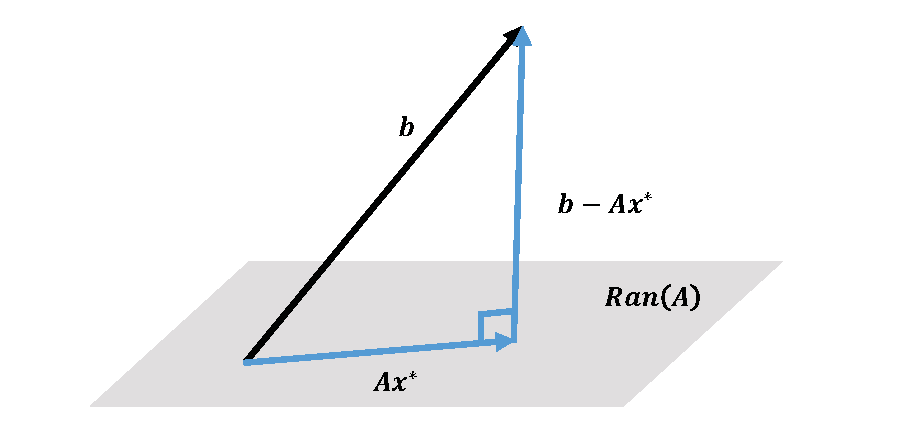
\includegraphics[width=13cm]{images/LSM.eps}\\
  \caption{最小二乘解的几何含义}\label{fig:LSM}
\end{figure}

通常$QR$算法比较稳定,是求解最小二乘问题的首选方法,特别是当$A$条件数较大(病态)时。

\subparagraph{奇异值分解法}
设$A\in\mathbb{R}^{n \times n}$列满秩,$A=U\begin{bmatrix}\Sigma \\ 0 \end{bmatrix}V^T$是$A$的奇异值分解。令$U_n$为$U$的前$n$列组成的矩阵,即$U=[U_n , \tilde{U}]$,则
\begin{displaymath}
\begin{aligned}
\Arrowvert Ax-b \Arrowvert_2^2 &= \Biggl\Arrowvert U\begin{bmatrix}\Sigma \\ 0 \end{bmatrix}V^Tx-b \Biggl\Arrowvert_2^2 \\
&= \Biggl\Arrowvert \begin{bmatrix}\Sigma \\ 0 \end{bmatrix}V^Tx-[U_n , \tilde{U}]^Tb \Biggl\Arrowvert_2^2 \\
&= \Biggl\Arrowvert \begin{bmatrix}\Sigma V^Tx-U_n^Tb \\ -\tilde{U}^Tb \end{bmatrix} \Biggl\Arrowvert_2^2 \\
&= \Arrowvert \Sigma V^Tx-U_n^Tb \Arrowvert_2^2 + \Arrowvert \tilde{U}^Tb \Arrowvert_2^2 \\
& \geq \Arrowvert \tilde{U}^Tb \Arrowvert_2^2
\end{aligned}
\end{displaymath}
等号当且仅当$\Sigma V^Tx-U_n^Tb=0$时成立,即
$$x=(\Sigma V^T)^{-1}U_n^Tb=V \Sigma ^{-1}U_n^Tb.$$
这就是线性最小二乘的解。

\section{非对称特征值问题}
设$A\in\mathbb{R}^{n \times n}$是一个非对称稠密矩阵,计算$A$的全部特征值和特征向量的方法主要有:
\begin{itemize}
  \item 幂迭代法
  \item 位移策略与反迭代技巧
  \item 正交迭代
  \item QR算法和实用QR算法
\end{itemize}
\paragraph{幂迭代}
幂迭代是计算特征值和特征向量的一种简单易用的方法,这种方法只能计算最特征值及对应的特征向量;并且幂迭代算法的收敛速度取决于$\arrowvert \lambda_2/\lambda_1 \arrowvert$的大小,$\arrowvert \lambda_2/\lambda_1 \arrowvert$ 越小,收敛越快。

\paragraph{反迭代}
既然幂迭代算法的收敛速度取决于$\arrowvert \lambda_2/\lambda_1 \arrowvert$的大小,容易想到的方法就是\textcolor[rgb]{0.00,0.07,1.00}{唯一策略},即将计算$A$的特征值转化为计算$A-\sigma I$的特征值,即先对$A$做一个位移,这里$\sigma$是一个给定的数,称为\textcolor[rgb]{0.00,0.07,1.00}{位移}(shift),为了使$A-\sigma I$具有更快的收敛速度,$\sigma$要满足两个条件:
\begin{enumerate}[(1)]
  \item $\lambda_1-\sigma$是$A-\sigma I$的模最大特征值
  \item $\max \limits_{2 \leq i \leq n}\arrowvert \frac{\lambda_i-\sigma}{\lambda_1-\sigma} \arrowvert$尽可能的小。
\end{enumerate}
位移策略在特征值计算中非常重要,主要是用在反迭代算法和QR迭代算法中。
\smallskip
如果将幂迭代算法作用在$A^{-1}$上,则课求出$A$的模最小的特征值,事实上,结合这种思想和位移策略,我们就能计算矩阵的任意特征值。

\paragraph{正交迭代}
幂迭代和反迭代只能同时计算一个特征对,如果想同时计算多个特征对,可以采用多个初始向量进行迭代。正交迭代算法正是应用这种思想,它能够计算$A$的一个不变子空间,从而可以同时计算出多个特征值。

\begin{algorithm}[H]
\caption{正交迭代算法}
\begin{algorithmic}[1]
  \State Choose an $n \times p$ column orthogonal matrix $Z_0$
  \State set $k=0$
  \State while not convergence do
  \State \qquad compute $Y_{k+1}=AZ_k$
  \State \qquad $Y_{k+1}=Z_{k+1}\hat{R}_{k+1}$    %QR分解
  \State \qquad $k=k+1$
  \State end while
\end{algorithmic}
\end{algorithm}

\paragraph{QR迭代}
QR迭代算法的基本思想是通过不断的正交变换,将$A$转换为上三角形式。
\begin{algorithm}[H]
\caption{QR迭代算法}
\begin{algorithmic}[1]
  \State Set $A_1=A$ and $k=1$
  \State while not convergence do
  \State \qquad $A_k=Q_kR_k$     %QR分解
  \State \qquad compute $A_{k+1}=R_kQ_k$
  \State \qquad $k=k+1$
  \State end while
\end{algorithmic}
\end{algorithm}
在该算法中有$A_{k+1}=R_kQ_k=(Q_k^TQ_k)R_kQ_k=Q_k^T(Q_kR_k)Q_k=Q_k^TA_kQ_k$,最终的迭代有$A_{k+1}=Q_k^TAQ_k^T$;需要指出的是$A_{k+1}$的对角线以上元素不一定收敛,但是$A_{k+1}$的对角线元素是收敛到特征值的,其收敛速度取决于$\max\limits_{1 \leq i \leq n}\arrowvert \frac{\lambda_{i+1}}{\lambda_i} \arrowvert$的大小。
\bigskip
为了加快QR迭代的收敛速度,可以采用位移策略和反迭代思想。
\begin{algorithm}[H]
\caption{带位移的QR迭代算法}
\begin{algorithmic}[1]
  \State Set $A_1=A$ and $k=1$
  \State while not convergence do
  \State \qquad Choose a shift $\sigma_k$
  \State \qquad $A_k-\sigma_kI=Q_kR_k$     %QR分解
  \State \qquad compute $A_{k+1}=R_kQ_k+\sigma_kI$
  \State \qquad $k=k+1$
  \State end while
\end{algorithmic}
\end{algorithm}

\paragraph{带位移的隐式QR迭代}
QR迭代运算中需要考虑的另一个重要问题就是运算量:每一步迭代需要做一次QR分解和矩阵乘积,运算量$\mathcal{O}(n^3)$。即使每计算一个特征值只需迭代一步,计算所有的特征值也需要$\mathcal{O}(n^4)$的运算量。为了将总运算量从$\mathcal{O}(n^4)$减小到$\mathcal{O}(n^3)$,需要用到Hessenberg矩阵。
具体步骤如下:首先通过相似变换将$A$转化为一个上$Hessenberg$矩阵,然后再对这个Hessenberg矩阵实施\textcolor[rgb]{0.00,0.07,1.00}{隐式QR迭代}。所谓隐式QR迭代,就是在QR迭代中,我们不需要进行显示的QR分解,这样就可以将QR迭代的每一步运算量从$\mathcal{O}(n^3)$降低到$\mathcal{O}(n^2)$。从而将总的运算量降低到$\mathcal{O}(n^3)$。

\paragraph{Hessenberg存在定理}
设$H=(h_{ij})\in\mathbb{R}^{n \times n}$,则存在正交矩阵$Q\in\mathbb{R}^{n \times n}$,使得$QAQ^T$是上Hessenberg矩阵。\newline

\textcolor[rgb]{0.00,0.07,1.00}{上Hessenberg矩阵一个很重要的性质就是在QR迭代中保持形状不变。}
\paragraph{Hessenberg矩阵QR迭代不变性}
设$A\in\mathbb{R}^{n \times n}$是非奇异上Hessenberg矩阵,其QR分解为$A=QR$,则$\tilde{A}\triangleq RQ$也是上Hessenberg矩阵。\newline

在QR迭代中,我们需要先做QR分解$A_k=Q_kR_k$,然后再计算$A_{k+1}=R_kQ_k$。但事实上,我们可以将这个过程进一步简化,即不用计算$A_k$的QR分解,可以直接计算$A_{k+1}$。这就是\textcolor[rgb]{0.00,0.07,1.00}{隐式QR分解}。隐式分解的理论基础是隐式Q定理(Implicit Q Theorem)

\paragraph{Implicit Q Theorem}
设$H=Q^TAQ\in\mathbb{R}^{n \times n}$是一个不可约上Hessenberg矩阵,其中$Q \in \mathbb{R}^{n \times n}$是正交矩阵,则$Q$的第2至第$n$列均有$Q$的第一列唯一确定(可相差一个符号)\newline

意思就是不用计算$A_k$的QR分解,可以直接计算$A_{k+1}$,就需要找到它们之间的迭代关系,由隐式Q定理可以找到$\tilde{Q}_k$使得其第一列与$Q_k$的第一列相等,且$\tilde{Q}_kA_k\tilde{Q}_k$为上Hessenberg矩阵,且有隐式定理可知$\tilde{Q}_k=WQ_k$,其中$W=diag(1,\pm 1,\cdots,\pm 1)$。于是
$$\tilde{Q}_kA_k\tilde{Q}=W^TQ^T_kA_kQ_kW=W^TA_{k+1}W$$
又$W^TA_{k+1}W$与$A_{k+1}$相似,且对角线元素相等,其它元素最多相差一个符号,故不影响收敛性,对角线元素收敛到$A$ 的特征值。因此在QR迭代算法中,可以用$\tilde{Q}_kA_k\tilde{Q}_k$替代$Q^T_kA_kQ_k$。这就是隐式QR迭代的基本思想。\newline

在实际的计算中$\tilde{Q}_k$是一系列Givens变换的乘积。
\end{flushleft}

\section{对称特征值问题}
\begin{flushleft}
设$A \in \mathbb{R}^{n \times n}$是对称矩阵。在计算$A$的特征值和特征向量是,我们可以充分利用$A$的堆成结构,一方面尽可能地减少运算,另一方面也构造出更快速高效的算法。\newline

关于对称矩阵的特征值和特征向量,目前常用的算法有:
\begin{itemize}
  \item \textcolor[rgb]{0.00,0.07,1.00}{Jacobi迭代:}最古老的算法,收敛速度慢但精度高,且适合并行计算。
  \item \textcolor[rgb]{0.00,0.07,1.00}{Rayleigh商迭代:}利用Rayleigh商作为位移和反迭代算法,一般具有三次收敛性。
  \item \textcolor[rgb]{0.00,0.07,1.00}{对称QR迭代:}如果对称三对角矩阵的所有特征值,则该算法是目前最快的算法(运算量$\mathcal{O}(n^2)$)。如果需要计算所有的特征值和特征向量,则运算量约为$6n^3$。
  \item \textcolor[rgb]{0.00,0.07,1.00}{分而治之(Divide-and-Conquer):}计算对称三对角矩阵的特征值和特征向量的一种快速算法。基本思想是将大矩阵分解成小矩阵,然后利用递推的思想求特征值和特征向量,在最坏的情形下,运算量为$\mathcal{O}(n^3)$,但在实际中,平均为$\mathcal{O}(n^{2.3})$。如果使用快速多极子算法(FMM)后,理论上运算量可降低到$\mathcal{O}(n\log^pn)$,其中$p$是一个较小的整数。
  \item \textcolor[rgb]{0.00,0.07,1.00}{对分法和反迭代:}对分法主要求解对称三对角矩阵在某个区间中的特征值,运算量约为$\mathcal{O}(kn)$,其中$k$为所需计算的特征值的个数;反迭代用于计算特征向量,在最佳情况下,即特征值“适当分离”时,运算量约为$\mathcal{O}(kn)$,但在最差情况下,即特征值成串靠在一起时,运算量约为$\mathcal{k^2n}$。
\end{itemize}
\end{flushleft}

\section{奇异值分解}
\begin{flushleft}
奇异值分解(SVD)具有十分广泛的应用背景,计算一个矩阵$A$的奇异值分解的算法通常分为以下几个步骤(Jacobi算法除外):
\begin{enumerate}[1.]
  \item 将$A$二对角化:$B=U_1^TAV_1$,其中$B$为上二对角矩阵,$U_1$,$V_1$为正交阵。
  \item 计算$B$的SVD:$B=U_2\Lambda V_2^T$,其中$\Lambda$为对角阵,$U_2$,$V_2$为正交阵。
  \item 合并得到$A$的SVD:$A=U_1BV_1^T=(U_1U_2)\Lambda (V_1V_2)^T$。
\end{enumerate}

\paragraph{二对角化}
对角矩阵可以通过一系列的Householder变化转化为对称三对角矩阵。对一般的矩阵$A \in \mathbb{R}^{n \times n}$,我们也可以通过Householder变换,将其转化为二对角矩阵,即计算正交矩阵$U_1$和$V_1$使得
$$U_1^TAV_1=B$$
其实$B$是一个实(上)二对角矩阵。这个过程就称为\textcolor[rgb]{0.00,0.07,1.00}{二对角化}。\newline

有了$U_1^TAV_1=B$后,可以得到
$$A^TA=(U_1BV_1^T)^T(U_1BV_1^T)=V_1B^TBV_1^T$$
由于$B^TB$是对称三对角的,所以就相当于将$A^TA$三对角化。\newline

整个二对角的运算量$4mn^2+4m^2n-4n^3/3$,若不需要计算$U_1$和$V_1$,则运算约为$4mn^2-4n^3/3$。

\paragraph{二对角矩阵的奇异值分解}
设$B \in \mathbb{R}^{n \times n}$是一个二对角矩阵
$$
B=
\begin{bmatrix}
a_1 & b_1 &  &  \\
    & \ddots & \ddots &  \\
    &     & \ddots & b_{n-1} \\
    &     &        & a_n
\end{bmatrix},
$$
下面三种方法可将计算$B$的SVD转化成计算对称三对称矩阵的特征分解:
\begin{enumerate}[(1)]
  \item 令$A=\begin{bmatrix}0 & B^T \\ B & 0\end{bmatrix}$,置换阵$P=[e_1,e_{n+1},e_2,e_{n+2},\cdots,e_n,e_{2n}]$,则$T_{ps}=P^TAP$是对称三对角矩阵,且$T_{ps}$的注对角线元素全为0,次对角线元素为$a_1,b_1,a_2,b_2,\cdots,a_{n-1},b_{n-1},a_n$。若$(\lambda_i,x_i)$是$T_{ps}$的一个特征对,则
      $$\lambda_i=\pm \sigma_i, \qquad Px_i=\frac{1}{\sqrt{2}}\begin{bmatrix}v_i \\ \pm u_i\end{bmatrix},$$
      其中$\sigma_i$为$B$一个奇异值,$u_i$和$v_i$分别为对应的左和右奇异向量。
  \item 令$T_{BB^T}=BB^T$,则
      $$
      T_{BB^T}=
      \begin{bmatrix}
      a_1^2+b_1^2 & a_2b_1 &        &          \\
      a_2b_1      & \ddots & \ddots &          \\
                  & \ddots & a_{n-1}^2+b_{n-1}^2 & a_nb_{n-1} \\
                  &        & a_nb_{n-1}          & a_n^2
      \end{bmatrix}
      $$
      $T_{BB^T}$的特征值为$B$的奇异值的平方,且$T_{BB^T}$的特征向量为$B$的左奇异向量。
  \item 令$T_{B^TB}=B^TB$,则
    $$
    T_{B^TB}=
      \begin{bmatrix}
      a_1^2 & a_1b_1 &        &          \\
      a_1b_1      & a_2^2+b_1^2 & \ddots &          \\
                  & \ddots & \ddots & a_{n-1}b_{n-1} \\
                  &        & a_{n-1}b_{n-1}          & a_n^2+b_{n-1}^2
      \end{bmatrix}
    $$
    $T_{B^TB}$的特征值为$B$的奇异值的平方,且$T_{B^TB}$的特征向量为$B$的右奇异向量。
\end{enumerate}

理论上,可以直接使用QR迭代、分而治之法或带反迭代的对分法,计算三对角矩阵$T_{ps}$,$T_{BB^T}$,$T_{B^TB}$的特征值和特征向量。但这种做法并不是最好的。
\begin{enumerate}[(1)]
  \item 对$T_{ps}$做QR迭代并不划算,因为QR迭代计算所有的特征值和特征向量,而事实上只要计算正的特征值即可。
  \item 直接构成$T_{BB^T}$,$T_{B^TB}$是数值不稳定的,事实上,这样做可能会使得$B$的小奇异值的精度丢失一半。
\end{enumerate}

\textcolor[rgb]{0.00,0.07,1.00}{下面算法比较实用:}
\begin{enumerate}[1.]
  \item Golub-Kahan SVD算法:Golub和Kahan于1965年提出,主要思想是将带位移的对称QR迭代算法隐式地用到$B^TB$上,在该算法中,并不需要显示地把$B^TB$计算出来。
  \item dqds算法:Fernando和Parlett于1994年提出,主要思想是对$B^TB$进行Cholesky迭代,可以看做是LR迭代算法的改进。由于LR迭代算法在一定条件下与对称QR算法是等价的,因此该算法也可以看作是QR迭代的变形。
  \item 分而治之算法:该算法是计算$\geq 25$的矩阵的所有奇异值和奇异向量的最快算法,但是不能保证小奇异值的相对精度。
  \item 对分法和反迭代:主要用于计算某个区间的奇异值和奇异向量,能保证较高的相对精度。
  \item Jacobi迭代:可隐式地对$AA^T$或$A^TA$实施对称Jacobi迭代,能保证较高的精度。2008年Z.Drma$\check{c}$和K.Veseli$\acute{c}$改进了最初的Jacobi算法。
\end{enumerate}
\end{flushleft}

\section{Krylov子空间迭代算法}
\begin{flushleft}
子空间迭代算法的基本思想是在一个维数较低的子空间中寻找解析解的一个“最佳”近似。子空间迭代算法的主要过程可以分解为下面三个步骤:
\begin{enumerate}[(1)]
  \item 寻找合适的子空间
  \item 在改子空间中求“最佳近似”
  \item 若这个近似解满足精度要求,则停止计算;否则重新构造一个新的子空间,并返回第(2)步
\end{enumerate}

明显地有两个关键点需要解决:
\begin{enumerate}[(1)]
  \item 如何选择和更新子空间
  \item 如何在给定的子空间中寻找“最佳近似”
\end{enumerate}

\paragraph{Arnoldi过程与Lanczos过程}
设$A \in \mathbb{R}^{n \times n}$,$r \in \mathbb{R}^n$,则由$A$和$r$生成的Krylov子空间为
$$\mathcal{K}_m(A,r)=span{r,Ar,A^2r,\cdots,A^{m-1}r}, \qquad m \leq n$$
通常简记为$\mathcal{K}_m$。\newline

设解析解在$\mathcal{K}_m$中的“最佳近似”为$x^{(m)}$。令$v_1,v_2,\cdots,v_m$是$\mathcal{K}_m$的一组基,则$\mathcal{K}_m$中的任意向量$x$均可表示为
$$x=y_1v_1+y_2v_2+\cdots+y_mv_m=V_my$$
其中$y=[y_1,y_2,\cdots,y_m]^T$为线性标出系数,$V_m=[v_1,v_2,\cdots,v_m]$。于是寻找“最佳近似”$x^{(m)}$就转化为
\begin{enumerate}[(1)]
  \item 寻找一组适合的基$v_1,v_2,\cdots,v_m$
  \item 求出$x^{(m)}$在这组基下的线性标出系数$y^{(m)}$
\end{enumerate}
\end{flushleft}
\end{document}
